\documentclass[sigplan]{acmart}

\settopmatter{printfolios=true,printccs=true,printacmref=false}
\renewcommand\footnotetextcopyrightpermission[1]{}
\pagestyle{plain}
\raggedbottom
\setlength{\emergencystretch}{2em}

\begin{document}

\title{World-Oriented Programming:\\Executable World Description Through Space, Time, and Constraints}
\shorttitle{World-Oriented Programming}

\author{Ibuki Nagase}
\affiliation{
  \institution{Osaka Electro-Communication University}
  \country{Japan}
}
\email{contact@enludus.com}

\begin{abstract}
This paper proposes World-Oriented Programming, a programming paradigm in which executable systems are described as worlds rather than as instruction sequences.
The proposal is motivated by a persistent mismatch between human spatial-temporal reasoning and conventional programming practice, especially in domains such as simulation, geometry, interactive environments, and world-based game logic.
In the proposed model, entities, spatial relations, temporal development, and logical constraints are represented directly, while execution is treated as the evolution of a constrained world over time.

The contribution of this paper is not a claim of mature generality.
Rather, it is a claim that this representational shift is already coherent enough to be instantiated in a small executable system.
The current prototype combines declarative world description, update-free temporal progression, constraint-first validity handling, and local synchronization at interaction points.
Three executable scenarios and a minimal visual round-trip are used as worked examples: a bouncing-sphere world, a forbidden-region world, a two-body collision world, and a viewer path from diagrammatic drafting to execution.
Together they show that simple spatial-temporal systems can already be expressed without user-authored update loops, that contradictions can be modeled as violations of world laws, that independently evolving entities can synchronize only when interaction occurs, and that visual arrangement can already participate in the same execution pipeline.
\end{abstract}

\begin{CCSXML}
<ccs2012>
<concept>
<concept_id>10011007.10011006.10011039</concept_id>
<concept_desc>Software and its engineering~Domain specific languages</concept_desc>
<concept_significance>500</concept_significance>
</concept>
<concept>
<concept_id>10011007.10011006.10011041</concept_id>
<concept_desc>Software and its engineering~Constraint and logic languages</concept_desc>
<concept_significance>500</concept_significance>
</concept>
<concept>
<concept_id>10003120.10003123.10011759</concept_id>
<concept_desc>Human-centered computing~Visual languages</concept_desc>
<concept_significance>300</concept_significance>
</concept>
<concept>
<concept_id>10010147.10010257.10010293</concept_id>
<concept_desc>Computing methodologies~Simulation environments</concept_desc>
<concept_significance>300</concept_significance>
</concept>
</ccs2012>
\end{CCSXML}

\ccsdesc[500]{Software and its engineering~Domain specific languages}
\ccsdesc[500]{Software and its engineering~Constraint and logic languages}
\ccsdesc[300]{Human-centered computing~Visual languages}
\ccsdesc[300]{Computing methodologies~Simulation environments}

\keywords{World-Oriented Programming, declarative worlds, spatial-temporal programming, local synchronization}

\maketitle

\input{main-body.tex}

% arXiv upload entry point: embed the generated bibliography output directly.
\documentclass[sigplan,review,anonymous]{acmart}

\settopmatter{printfolios=true,printccs=true,printacmref=false}
\renewcommand\footnotetextcopyrightpermission[1]{}
\pagestyle{plain}
\raggedbottom
\setlength{\emergencystretch}{2em}

\begin{document}

\title{World-Oriented Programming:\\Executable World Construction and Law Through Space, Time, and Constraints}
\shorttitle{World-Oriented Programming}

% Anonymous review package:
% keep the manuscript anonymous for Phase E.
% When preparing a named submission or camera-ready version,
% replace the anonymous class option and add author/affiliation blocks here.

\begin{abstract}
This paper proposes World-Oriented Programming, a programming paradigm in which executable systems are constructed as worlds with explicit laws rather than authored as instruction sequences.
The proposal is motivated by a persistent mismatch between human spatial-temporal reasoning and conventional programming practice, especially in domains such as simulation, geometry, interactive environments, and world-based game logic.
In the proposed model, programs construct worlds by declaring entities, spatial relations, temporal development, and logical constraints directly, while execution is treated as the admissible evolution of those worlds over time.

The contribution of this paper is not a claim of mature generality.
Rather, it is a claim that executable world construction and explicit world law are already coherent enough to be instantiated together in a small executable system.
The current prototype combines declarative world description, update-free temporal progression, constraint-first validity handling, and local synchronization at interaction points.
Three executable scenarios and a minimal visual round-trip are used as worked examples: a bouncing-sphere world, a forbidden-region world, a two-body collision world, and a viewer path from diagrammatic drafting to execution.
Together they show that simple spatial-temporal systems can already be expressed by constructing worlds and stating laws rather than by authoring update procedures, that contradictions can be modeled as violations of world laws, that independently evolving entities can synchronize only when interaction occurs, and that visual arrangement can already participate in the same execution pipeline.
\end{abstract}

\begin{CCSXML}
<ccs2012>
<concept>
<concept_id>10011007.10011006.10011039</concept_id>
<concept_desc>Software and its engineering~Domain specific languages</concept_desc>
<concept_significance>500</concept_significance>
</concept>
<concept>
<concept_id>10011007.10011006.10011041</concept_id>
<concept_desc>Software and its engineering~Constraint and logic languages</concept_desc>
<concept_significance>500</concept_significance>
</concept>
<concept>
<concept_id>10003120.10003123.10011759</concept_id>
<concept_desc>Human-centered computing~Visual languages</concept_desc>
<concept_significance>300</concept_significance>
</concept>
<concept>
<concept_id>10010147.10010257.10010293</concept_id>
<concept_desc>Computing methodologies~Simulation environments</concept_desc>
<concept_significance>300</concept_significance>
</concept>
</ccs2012>
\end{CCSXML}

\ccsdesc[500]{Software and its engineering~Domain specific languages}
\ccsdesc[500]{Software and its engineering~Constraint and logic languages}
\ccsdesc[300]{Human-centered computing~Visual languages}
\ccsdesc[300]{Computing methodologies~Simulation environments}

\keywords{World-Oriented Programming, declarative worlds, spatial-temporal programming, local synchronization}

\maketitle

\section{Introduction}

Programming languages are usually organized around procedures, instruction order, and explicit state updates.
This design has proved effective for a vast range of software, but it sits awkwardly with problem domains that humans understand primarily in terms of space, relation, motion, and constraint.
When developers build simulations, game worlds, geometric systems, or interactive spatial models, they often begin from a mental picture of a world and its laws.
Yet mainstream implementations typically force that picture into control flow, frame loops, and manual state mutation.

This paper begins from the claim that this is a representational mismatch.
In many settings, the programmer's real intention is not best described as a procedure.
It is better described as a world: what exists, how it may evolve, what interactions matter, and what laws must never be violated.

We therefore explore an alternative paradigm: \emph{World-Oriented Programming}.
In this model, a program is an executable world description together with laws of admissible development.
The programmer specifies entities, spatial structure, temporal development, and logical constraints directly.
Execution is understood as world evolution under admissibility laws, not as running an instruction list.

The long-term vision is ambitious.
Ultimately, the project aims toward a computational environment in which diagrams, formulas, logical constraints, and execution all refer to the same underlying world model.
This paper, however, makes a narrower contribution.
It presents the paradigm, gives a first prototype, and asks whether three central ideas are already executable in a nontrivial but still deliberately small system:
\begin{enumerate}
\item worlds can evolve without user-authored update loops,
\item constraints can be expressed as world laws rather than imperative exception handlers, and
\item interaction can be localized to synchronization points rather than imposed globally.
\end{enumerate}

The paper's concrete contributions are:
\begin{enumerate}
\item a formulation of World-Oriented Programming as a paradigm centered on executable world construction and explicit world law rather than procedure,
\item a functioning prototype that combines declarative world description, constraint-first admissibility, and local synchronization, and
\item a first visual-logical interface in which diagrams, candidate world laws, execution, and contradiction reporting share one report pipeline.
\end{enumerate}

This framing fits an Onward!-style submission, where the key question is not whether a new idea has already reached mature generality, but whether it is conceptually meaningful, well argued, and supported by enough implementation to justify taking it seriously.

\section{Related Work}

World-Oriented Programming is not unprecedented in every dimension.
Its importance lies in the attempted integration of concerns that are usually split across separate communities.

Constraint Logic Programming provides one major antecedent because it treats constraints as part of the computational core rather than as post hoc checks \cite{jaffar1987clp}.
Functional Reactive Programming provides a major precedent on the temporal axis \cite{hudak1999frp,elliott1997fra}.
Modelica is perhaps the closest existing large-scale modeling relative because it supports declarative model execution without manually selecting variable-solving order \cite{modelica2023spec}.
The actor model is relevant for the asynchronous part of the proposal \cite{hewitt1973actor}.
GeoGebra and LabVIEW are useful practical precedents because they show that executable meaning can live in representations other than plain sequential text \cite{geogebra,ni2026labview}.

The clearest claim of this paper is therefore not that World-Oriented Programming is unprecedented in every dimension.
Rather, it explores a new synthesis: spatial world description, temporal evolution, constraints as laws, and local synchronization brought together inside a single executable language model.

\section{World-Oriented Programming Model}

\subsection{Programs as World Descriptions}

The central shift is to treat a program as a world definition rather than as a procedure.
In the proposed model, the programmer describes what entities exist, how they are situated in space, how they evolve in time, what constraints define admissible development, and which interactions require shared interpretation.
This changes the main question of programming from ``how do I update the state?'' to ``what kind of world is being defined?''

\subsection{First-Class Space, Time, and Constraint}

The model assumes that space, time, and constraint should be part of the semantic core rather than merely library conventions.
Even in the current prototype, the primary language objects are spheres, planes, regions, motion descriptors, and collision or admissibility constraints.

Time is not authored through explicit repeated updates.
Instead, the runtime advances the world in response to observation and interaction demands.
Constraints are not framed as secondary checks.
They are treated as laws of admissible world development.

\subsection{Global Asynchrony and Local Synchronization}

The execution model aims for global asynchrony with local synchronization.
Independent entities should not need to remain in permanent global lockstep.
They only need synchronized interpretation when the world's semantics require it.

In the current prototype, this idea appears in a simple but meaningful form.
Worlds are observed through snapshots at requested times, while multi-object interaction is only resolved when a declared interaction constraint becomes relevant.

\section{Toward an Operational Semantics}

The semantics work now underway sharpens the prototype intuition into an explicit staged model.
The current formulation distinguishes five layers:
time frontier and observation structure, event ordering, local synchronization scope, event versus enforcement transition, and final semantic consolidation.
The present paper does not yet attempt a theorem-level development.
It does, however, now have enough structure to present a genuine semantics trajectory rather than only an execution metaphor.

At the current level of formalization, a world at frontier $t$ can already be read as a tuple containing dynamic entities, static geometry, declared laws, an object-local progress function, a current state assignment, and the frontier itself.
Events and laws can likewise be treated as explicit semantic objects rather than implementation accidents, while admissibility can be stated as a predicate over the world at a given frontier.
This is still a lightweight formalization, but it is enough to move the discussion from conceptual vocabulary toward a reusable operational core.

\begin{figure}[t]
  \centering
  \small
  \setlength{\tabcolsep}{3pt}
  \renewcommand{\arraystretch}{1.15}
  \begin{tabular}{c c c c c c}
    \fbox{\parbox[c][1.8em][c]{0.10\columnwidth}{\centering $W_t$}} &
    $\Rightarrow$ &
    \fbox{\parbox[c][1.8em][c]{0.16\columnwidth}{\centering $ev = Next(W_t)$}} &
    $\Rightarrow$ &
    \fbox{\parbox[c][1.8em][c]{0.15\columnwidth}{\centering $Sync(ev)$}} &
    $\Rightarrow$ \\
    \multicolumn{6}{c}{} \\
    \fbox{\parbox[c][1.8em][c]{0.15\columnwidth}{\centering $W_t^{ev}$}} &
    $\Rightarrow$ &
    \fbox{\parbox[c][2.8em][c]{0.16\columnwidth}{\centering admissible\\ $W_t'$}} &
    \multicolumn{1}{c}{or} &
    \fbox{\parbox[c][2.8em][c]{0.14\columnwidth}{\centering failure\\ $W_t^{X}$}} &
    \\
  \end{tabular}

  \vspace{0.4em}

  \fbox{\parbox[c][2.1em][c]{0.68\columnwidth}{\centering observation frontier: $\mathrm{Obs}(W, t_{obs})$ is valid only after earlier event frontiers are resolved}}
  \caption{Semantics pipeline for the current \emph{sekai} model. A world at frontier $t$ yields a next event, a minimal synchronization carrier, and then either an admissible continuation or contradiction at the same frontier. Observation is defined over resolved frontiers rather than over a mandatory global frame loop.}
  \label{fig:semantics-pipeline}
\end{figure}

\subsection{Time Frontiers and Observation}

The working time model treats the world at a semantic frontier $t$ rather than as a sequence of user-authored frame updates.
Observation is expressed as a request for a coherent snapshot at some time $t_{obs}$.
This matters because it shifts temporal meaning away from a frame loop and toward a frontier-based interpretation of world state.
Figure~\ref{fig:semantics-pipeline} summarizes the current staged reading of that process.

In this view, the runtime is not repeatedly asked to ``run the next update.''
It is asked to provide an admissible world at a requested semantic frontier, resolving whatever earlier event frontiers must be settled first.

\subsection{Event Ordering and Local Synchronization}

Candidate events are selected from the current frontier by an ordering rule that combines earliest-time selection with a semantic priority and a deterministic tie-breaker.
The point of this rule is not only determinism.
It is to preserve causal meaning when several events become simultaneously relevant.

Once an event is selected, only its minimal synchronization carrier needs to be brought to a common frontier.
That carrier includes the event participants and the smallest dependency context needed to interpret the event correctly.
This is the semantic core of the claim ``global asynchrony with local synchronization.''

\subsection{Event, Enforcement, and Contradiction}

The next transition is factored into event firing and admissibility enforcement.
An event first produces a post-event world at the same semantic frontier.
The law set is then used to determine whether that frontier admits a valid continuation.

In the admissible case, the world continues after any required repair.
In the inadmissible case, execution reaches contradiction at the same frontier instead of falling back to an out-of-band exception model.
This framing gives a clean reading to the runtime's current activity labels: fired, repaired, and contradicted.

The semantics draft can now also state these stages as compact rule blocks:
\emph{Select}, \emph{Sync}, \emph{Fire}, \emph{Enforce}, \emph{Contradict}, and \emph{Observe}.
That is still lighter than a full theorem-proof semantics, but it is already closer to an operational account than to a design metaphor.

\subsection{Deterministic Snapshots Without Global Lockstep}

This semantics direction lets the paper make a stronger claim than before:
deterministic snapshots need not come from mandatory global lockstep execution.
They can instead arise from deterministic event selection plus coherent local synchronization and admissibility handling.

The right next step is therefore not to over-claim finished theory, but to name the proof obligations that now matter most.
At least three are already visible:
snapshot determinism, causality preservation, and repair termination.
The present prototype does not yet prove them.
It does, however, make them explicit enough to become targets of the next semantics paper rather than vague future aspirations.

That claim is still only partially formalized.
Even so, it marks an important shift in the project.
\emph{sekai} is no longer described only as an implementation experiment.
It is beginning to take the shape of a language with an operational semantics.

\section{Prototype Architecture}

The prototype consists of five connected layers:
\begin{enumerate}
\item a small textual DSL,
\item a runtime core,
\item structured snapshot export,
\item an interactive viewer and draft editor, and
\item static figure generation.
\end{enumerate}

The textual DSL is implemented in \texttt{sekai}.
The runtime core is implemented in \texttt{orbis}.
The current system supports spheres, one static plane, an axis-aligned region model, velocity limits, forbidden regions, a first visibility law, and pairwise elastic collisions.

Execution begins by constructing a world from declarations.
The runtime then advances the relevant state to requested observation times, while resolving interaction events only when they become semantically relevant.
Users do not write an explicit frame loop.

JSON snapshot export provides a stable interface for later tools, including viewers and analysis scripts.
Those snapshots are already sufficient to generate paper-ready static figures directly from executable examples.

The browser-based viewer adds three capabilities that matter to the research argument.
First, it makes executable worlds inspectable through one spatial-temporal interface.
Second, it introduces a minimal diagram-aware editor that proposes floor reflection, collision, speed bounds, and forbidden-region exclusion.
Third, it closes a first round-trip path in which a draft scene is executed through the same runtime and then reloaded into the viewer.
The viewer is not presented as a polished end-user environment.
It is evidence that one world model can already support inspection, drafting, logical suggestion, execution, and contradiction display in one prototype loop.

\section{Prototype Evaluation}

This evaluation is intentionally modest.
It is not an attempt to prove that World-Oriented Programming is already superior to mature programming paradigms.
Rather, it asks whether explicit world construction plus explicit world law are coherent enough to support a first executable system whose behavior genuinely reflects the ideas the paper claims to embody.

The evaluation is organized around three questions:
\begin{enumerate}
\item Can a minimal world evolve without a user-authored update loop?
\item Can constraints be expressed as world laws rather than imperative exception handlers?
\item Can independent entities progress separately while synchronizing only at interaction points?
\end{enumerate}

\subsection{Evaluation Setup}

The prototype is evaluated through three executable scenarios written in the same DSL and executed by the same runtime:
\emph{bounce}, \emph{forbidden region}, and \emph{two-body collision}.
For each scenario, the runtime produces snapshots at explicitly requested observation times.
Those snapshots are exported as JSON and rendered into static figures.

This example-driven method is deliberate.
At the present stage, the paper is not trying to claim benchmark superiority or broad usability.
It is trying to establish semantic coherence: whether the paradigm's core claims can survive contact with an executable artifact.

\subsection{Compact Imperative Baseline}

The comparison target throughout this paper is the conventional style in which the same scenarios are written with explicit update loops, manual state mutation, and distributed guard logic.
For the bounce example, that baseline typically requires per-frame position updates plus explicit collision handling.
For the forbidden-region example, it requires imperative checks around movement or collision steps.
For the two-body case, it requires manual event detection and collision-response sequencing.
The current evaluation scaffold now also includes a first visibility pair, where \texttt{visible(A, B)} is contrasted with imperative line-of-sight checking against one or more occluding regions.
It now also includes a first visibility-conditioned pursuit pair, where line of sight changes which equally scored continuation is preferred.
It now also includes a first branching visibility world, where the same geometry switches a world between pursuit-like and search-like continuations.
It now also includes a first corridor-style visibility world, where several walls preserve or close a narrow line of sight and thereby change which continuation the world admits.
It now also includes a first time-varying corridor slice, where a moving target later enters or leaves that visibility channel and resolves a previously deferred world.
It now also includes a first multi-target visibility handoff, where the same deferred world resolves toward different pursuit continuations depending on which target later becomes visible.
It now also includes a first multi-agent visibility coordination slice, where one shared visibility change resolves several candidate-bearing entities at the same observation frontier.
It now also includes a first visibility network slice, where the same geometry assigns several agents to target-specific roles.
It now also includes a first staggered visibility network slice, where those role assignments can change across observation frontiers as line of sight changes.
It also now includes a first multi-surface channel world, where one sphere can reflect between several declared planes rather than only one global floor.
It now also includes a first plane-bounded wedge slice, where a slanted pair of planes keeps a sphere inside a non-axis-aligned admissible channel.
It now also includes a first bounded surface room slice, where several planes jointly define an admissible pocket through one explicit geometry law.
It now also includes a first reflective surface room slice, where several planes remain active as simultaneous contact boundaries.
It now also includes a first gated-surface slice, where one wall is traversable only through an explicit door aperture.
It now also includes a first time-varying gate slice, where that same aperture can remain closed until a later frontier and thereby alter whether a deferred continuation eventually crosses or is repaired back inside the current room.
It now also includes a first gate-conditioned branching slice, where the opening state of one doorway changes whether a deferred world later prefers `enter` or `wait`.
It now also includes a first multi-gate routing slice, where several delayed apertures can steer the same deferred world toward different exits.
It now also includes a first staggered room-network slice, where several entities can resolve through different gates at different observation frontiers.
It now also includes a first shifted-gate slice, where the aperture itself can later move into or out of alignment and thereby change whether a deferred world crosses the boundary or remains in place.
The present prototype does not yet prove that World-Oriented Programming is always shorter or faster.
It does show a consistent relocation of semantic burden: \emph{sekai} keeps world construction and admissibility law explicit, while imperative baselines bury both inside update loops, guard logic, and control-flow bookkeeping.

\subsection{Structural Comparison Snapshot}

The current Phase K scaffold also provides a small structural comparison against compact imperative baselines.
Table~\ref{tab:baseline-snapshot} reports three representative cases: basic world evolution, underdetermined convergence, and geometry-conditioned branching.
These numbers are intentionally modest rather than exhaustive.
They are included to show that the evaluation is already reproducible and that the current corpus consistently keeps world construction and law explicit while shifting specification effort away from loops, branches, and explicit update bookkeeping.

\begin{table}[t]
  \caption{Representative structural comparison between \emph{sekai} and compact imperative baselines.}
  \label{tab:baseline-snapshot}
  \centering
  \small
  \begin{tabular}{lrrrr}
    \toprule
    Scenario & LOC$_s$ & LOC$_i$ & Density$_s$ & Branch$_i$ \\
    \midrule
    bounce & 15 & 32 & 0.867 & 3 \\
    candidate deferred & 13 & 36 & 0.846 & 4 \\
    visibility pursuit world & 20 & 56 & 0.900 & 8 \\
    visibility corridor world & 28 & 62 & 0.929 & 9 \\
    surface channel & 18 & 34 & 0.889 & 4 \\
    surface room clamped & 22 & 61 & 0.955 & 5 \\
    surface room reflective & 26 & 41 & 0.846 & 6 \\
    surface gate clamped & 19 & 49 & 0.947 & 4 \\
    surface gate deferred & 23 & 67 & 0.826 & 7 \\
    surface gate branch & 24 & 68 & 0.792 & 6 \\
    surface gate route & 32 & 55 & 0.812 & 12 \\
    surface gate network & 51 & 83 & 0.765 & 20 \\
    surface gate shifted & 24 & 45 & 0.792 & 6 \\
    \bottomrule
  \end{tabular}
\end{table}

Across this first corpus, \emph{sekai} remains shorter and more declarative in structure, while the imperative versions spend more of their specification budget on explicit control and state-management machinery.
The point is not that these initial baselines are definitive.
It is that even the first scaffold already supports a stable narrative: once space, time, admissibility, and convergence are made first-class, the center of expression moves away from update logic and toward world description.

\subsection{Minimal Declarative Evolution}

The first scenario is a bouncing sphere described in the \emph{bounce} example.
The program declares a sphere, a floor plane, initial position and velocity, and a reflective collision law.
No user-authored update function is present.

\begin{figure}[t]
  \centering
  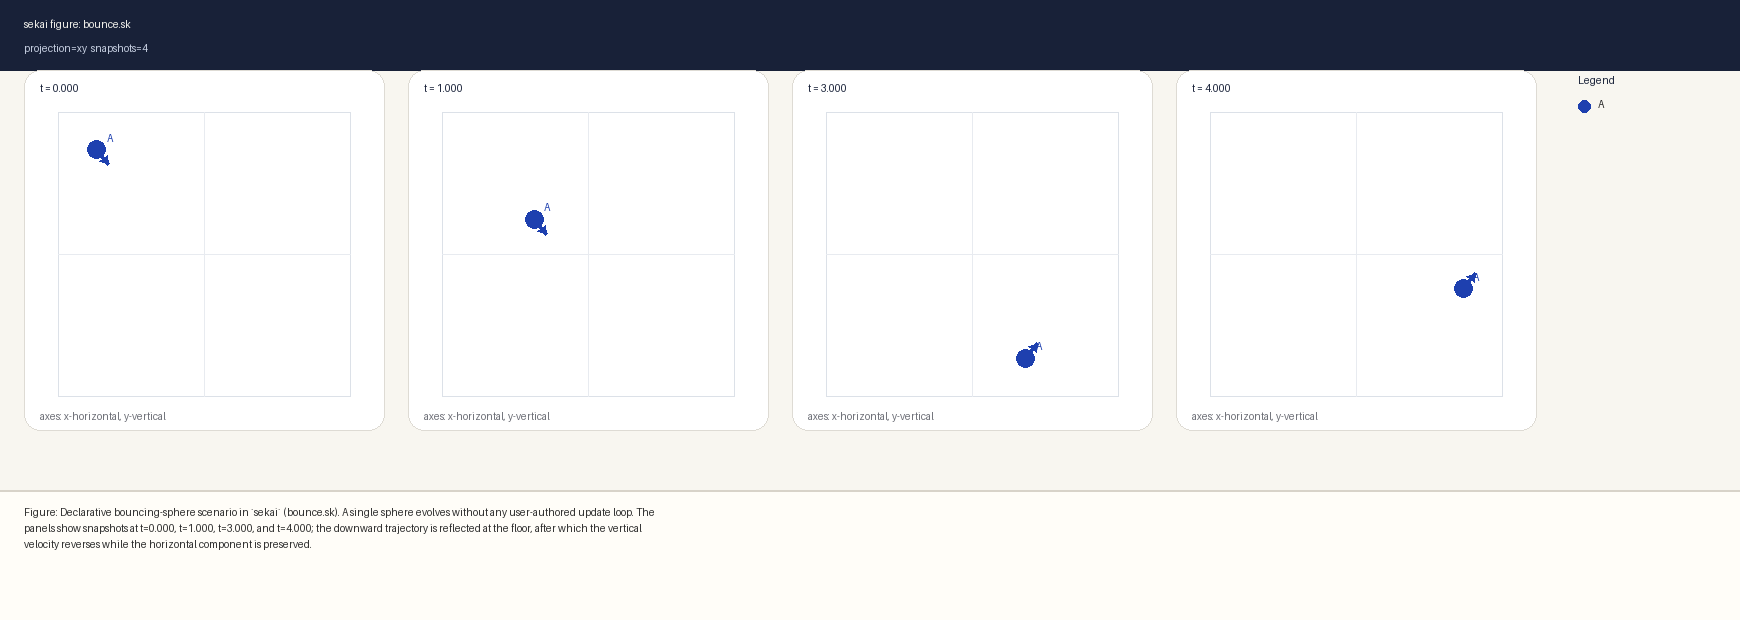
\includegraphics[width=\columnwidth]{../figures/bounce-xy.png}
  \caption{Declarative bouncing-sphere scenario in \texttt{sekai}. A single sphere evolves without a user-authored update loop. The panels show snapshots at $t=0.000$, $t=1.000$, $t=3.000$, and $t=4.000$.}
  \label{fig:bounce}
\end{figure}

Figure~\ref{fig:bounce} shows the resulting snapshot sequence.
The sphere first moves downward and then reflects at floor contact, reversing its vertical velocity while preserving the horizontal component.

\subsection{Constraint-First Contradiction Handling}

The second scenario is a forbidden-region world described in the \emph{forbidden region} example.
The user does not write imperative guard code around each movement step.
Instead, the world definition states that a sphere may not enter a specified region.

When the sphere reaches that region, the runtime reports the violation as a contradiction in world development.
This does not yet amount to a full constraint-solving framework, but it shows that invalid evolution can already be described declaratively and detected as a property of the modeled world.
Figure~\ref{fig:viewer-contradiction} shows the same idea in the visual interface: an adopted exclusion law is executed and then reported back as a contradiction in the same world-report loop.

\begin{figure*}[t]
  \centering
  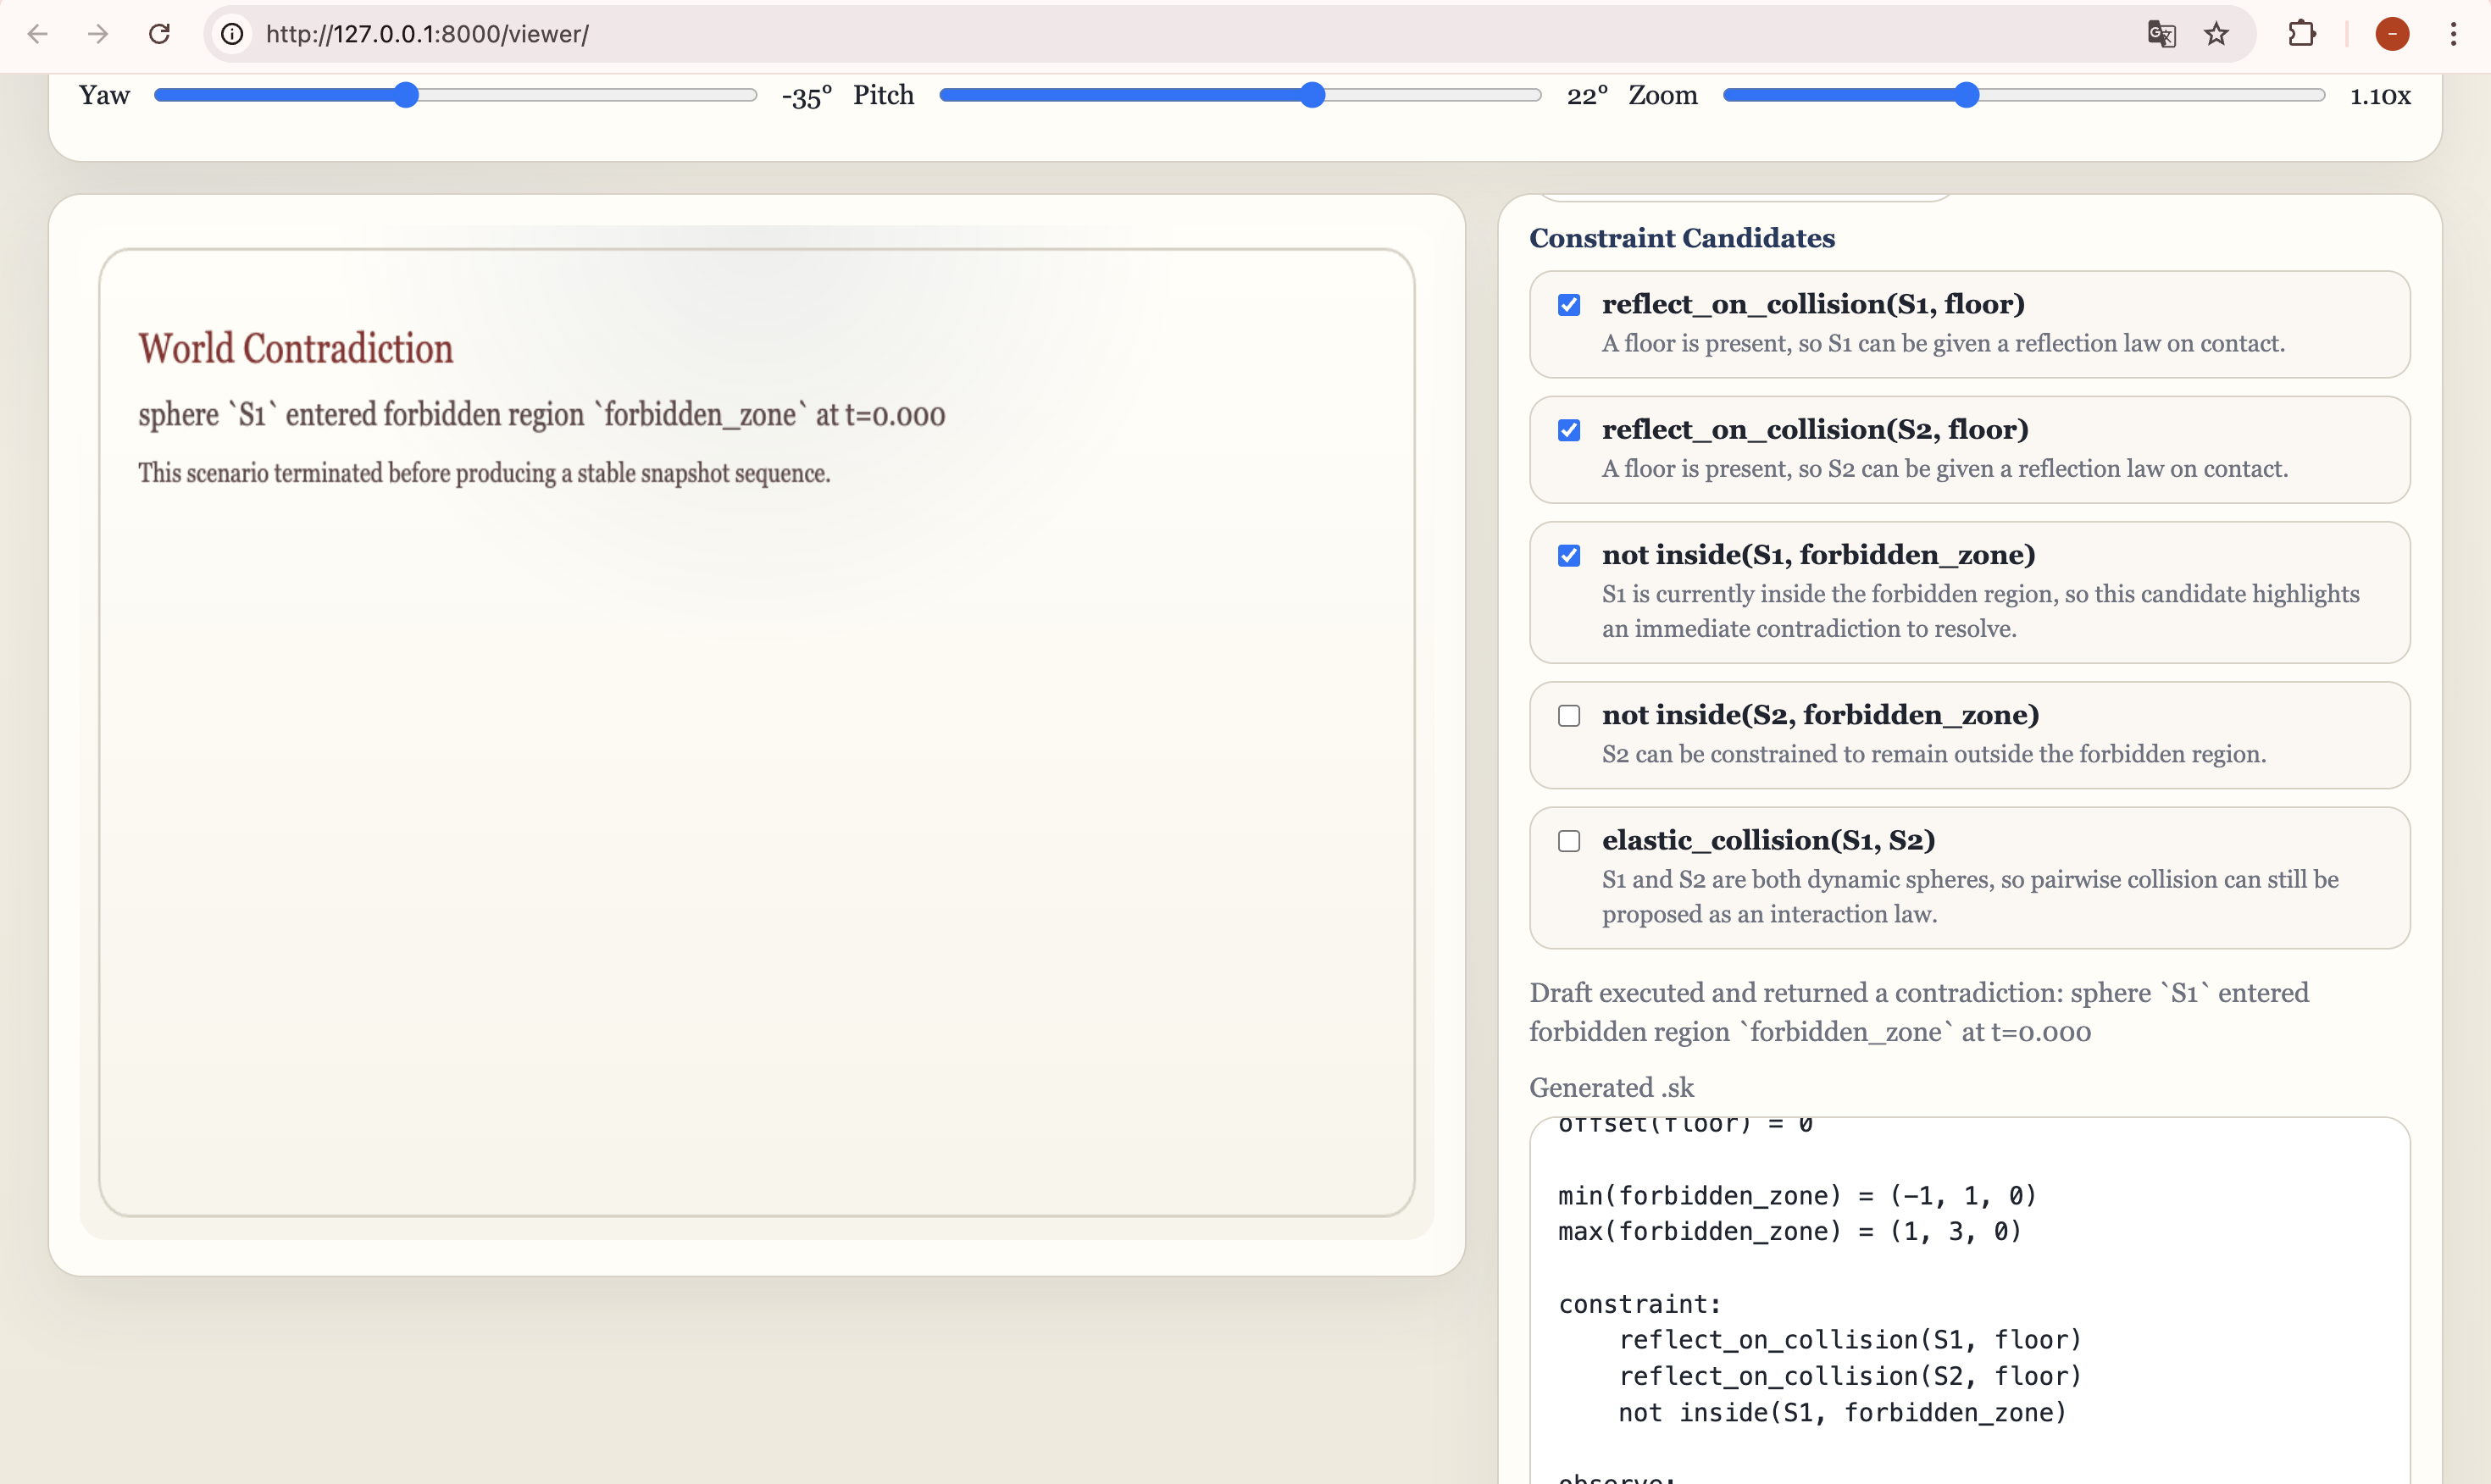
\includegraphics[width=0.9\textwidth]{../figures/viewer-04-contradiction-report-paper.png}
  \caption{Constraint violation as a world contradiction in the viewer. After enabling \texttt{not inside(S1, forbidden\_zone)}, execution fails with an explicit contradiction report.}
  \label{fig:viewer-contradiction}
\end{figure*}

\subsection{Local Synchronization}

The third scenario is a two-body collision world described in the \emph{two-body collision} example.
Two spheres move independently until an explicit elastic-collision rule becomes relevant.
Before contact, they follow separate trajectories.
At contact, a local synchronization event is resolved, after which the spheres continue with exchanged velocities.

\begin{figure*}[t]
  \centering
  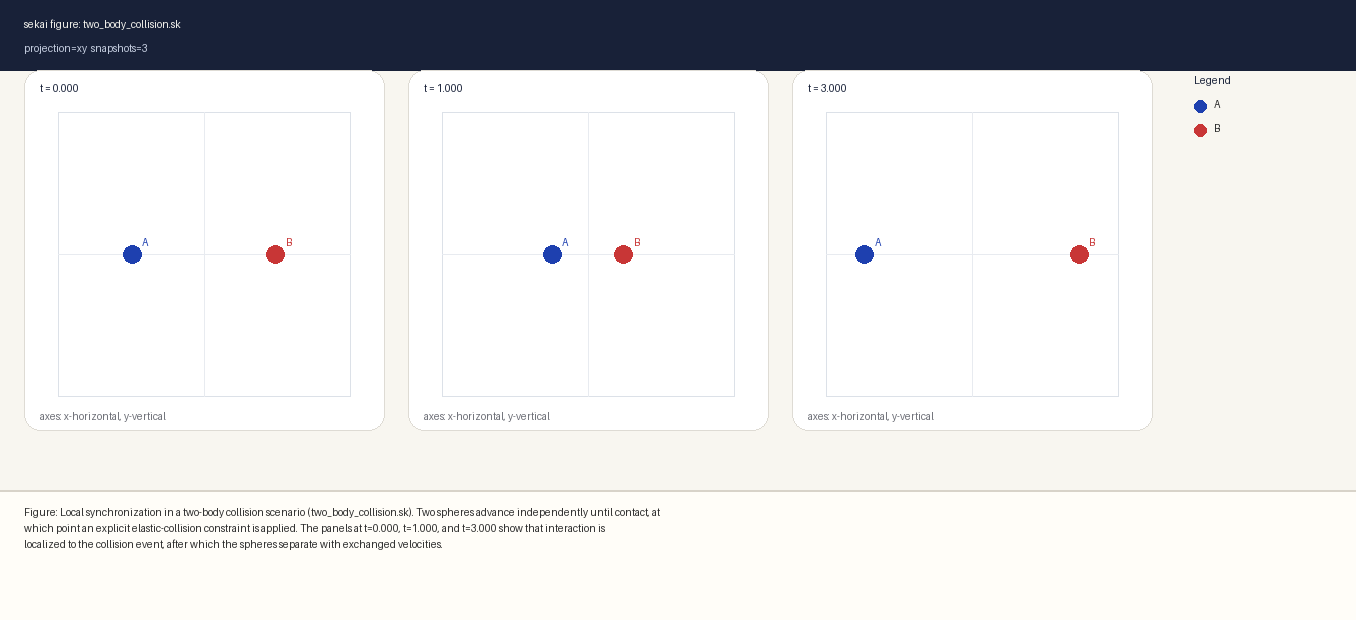
\includegraphics[width=0.9\textwidth]{../figures/two_body_collision-xy.png}
  \caption{Local synchronization in a two-body collision scenario. Two spheres advance independently until contact, where an explicit elastic-collision constraint is applied.}
  \label{fig:collision}
\end{figure*}

\subsection{Visual-Logical Round-Trip}

A user can place spheres in the viewer, enable a floor or forbidden region, inspect proposed constraints, and execute the generated draft through the same runtime.
The resulting report is then shown in the same interface.
This gives the prototype its first end-to-end visual-logical cycle: arrangement, candidate law selection, execution, and inspection.
That same draft layer can now also propose a small visibility-pursuit world, so the editor is beginning to surface geometry-conditioned action structure rather than only static laws.

\begin{figure*}[t]
  \centering
  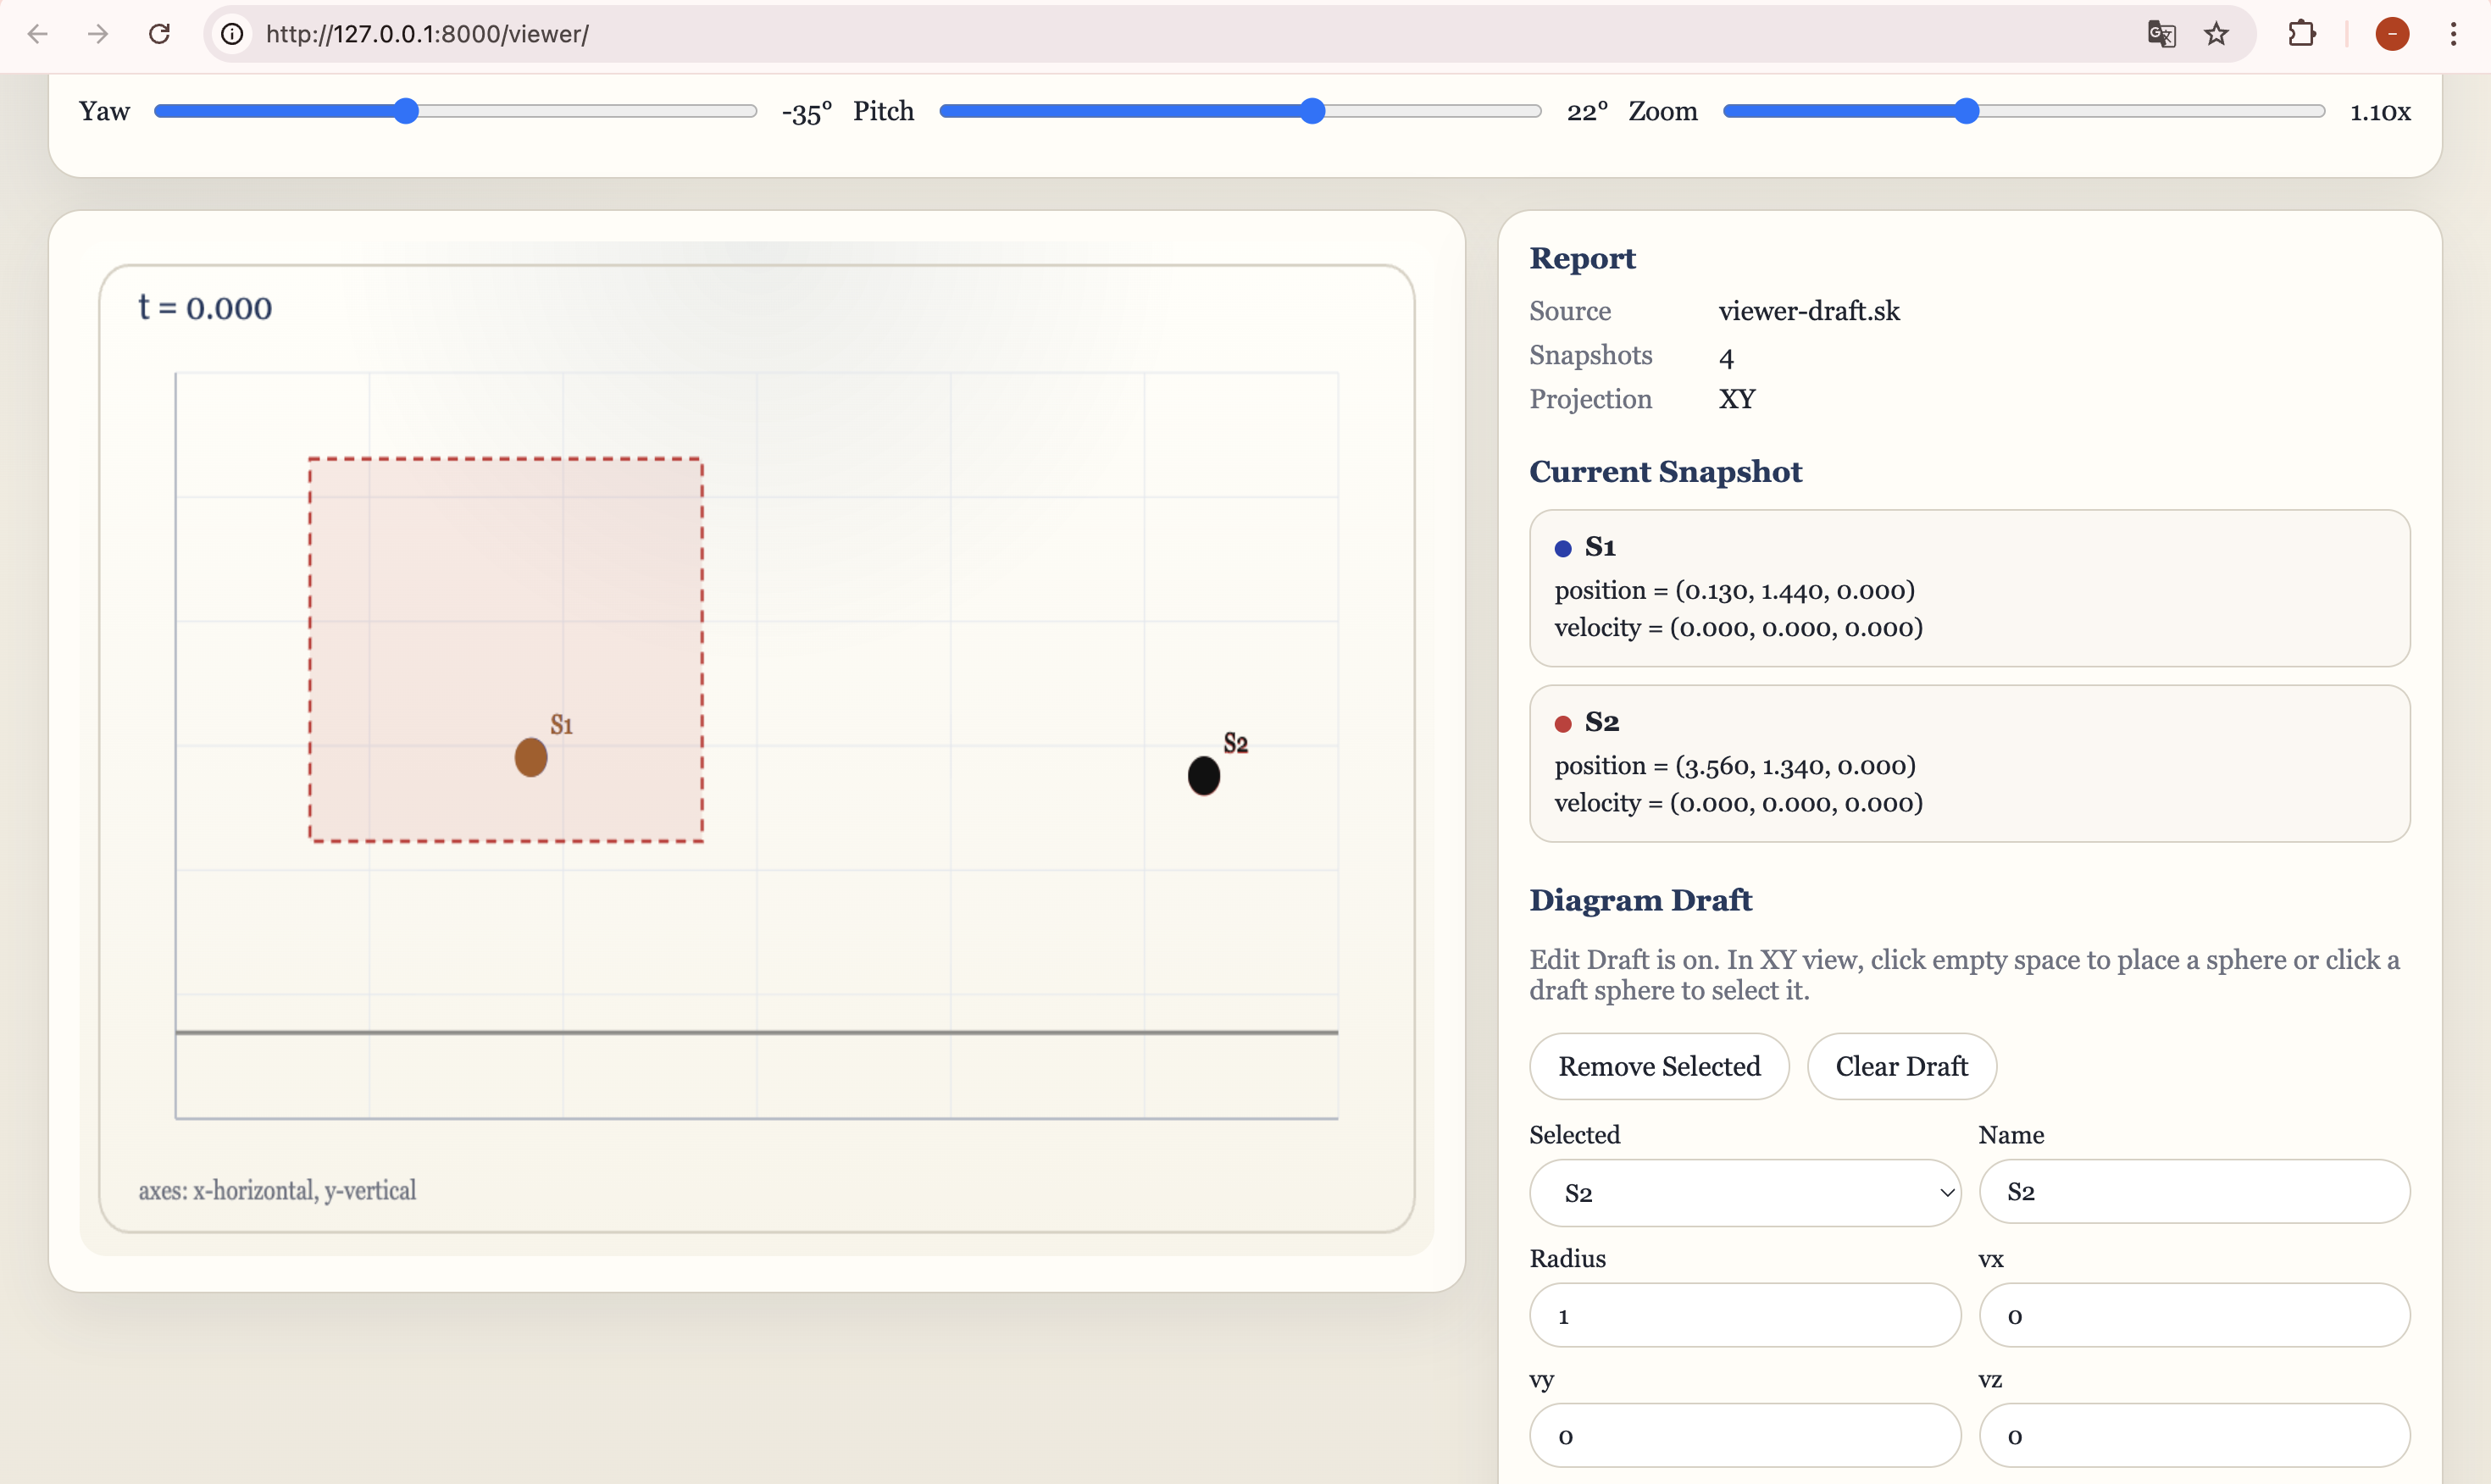
\includegraphics[width=0.9\textwidth]{../figures/viewer-03-roundtrip-result-paper.png}
\caption{Round-trip execution from diagram editing to world simulation. A draft scene is executed through \texttt{Run Draft}, after which the returned world report is displayed in the same interface.}
\label{fig:viewer-roundtrip}
\end{figure*}

\subsection{Visibility-Conditioned World Branching}

The richer-geometry direction is now beginning to produce its own executable pillar rather than only remaining future work.
In the current visibility slice, \texttt{visible(A, B)} is not only a contradiction condition.
It can also participate in action preference, so the same world can prefer a pursuit-like continuation when line of sight is clear and a search-like continuation when one or more occluding regions block visibility.
The current branch of that geometry work now also includes a first corridor-like scenario, where side walls preserve a narrow visibility channel and an inserted blocker closes it.
That same geometry can now vary across observation frontiers, so a deferred world may later resolve differently when the target enters or leaves the corridor's visibility channel.
The same setup can now also hand off convergence between several target-specific pursuit continuations, so geometry does not only decide whether pursuit is admissible, but also which pursuit the world should admit.
It can now also coordinate more than one deferred entity at once, so line of sight begins to look like a shared world condition that can align several continuations without introducing imperative synchronization logic.
The next small step beyond that is already visible in the prototype: geometry can assign several agents to target-specific roles inside the same visibility network, which makes line of sight look less like a local branch and more like a routing condition over world development.
That role assignment can now also be staggered across frontiers, so a visibility network need not collapse in one step; different agents can resolve at different times as the geometry evolves.
In parallel, a second geometry family is now beginning to appear: multiple surfaces with contact rules and plane-bounded spaces. The current prototype can already declare a small surface channel with a floor and ceiling and bind reflection laws to each plane independently, and it can now also keep a sphere inside a slanted plane-bounded wedge, repair it inside a bounded surface room, let it bounce inside that room through explicit geometry laws, or restrict crossing through a wall to one named gate aperture. That moves Phase J past the older assumption that the world contains only one meaningful contact surface or only axis-aligned admissible volumes.
That same geometry family can now also vary across frontiers, since a gate can remain closed until a later opening time and thereby change whether a deferred continuation eventually passes into the next space or is repaired back to the current side of the wall.
It can now also steer convergence directly, since the same gate state can decide whether the world keeps waiting or commits to room entry at the deferred frontier.

Figure~\ref{fig:visibility-pursuit} shows this emerging geometry path in one visual sequence.
The center panel is the editor-side world candidate, while the left and right panels show executed reports for the clear and occluded cases.
The key point is that the branching is still expressed as part of one world description pipeline rather than as distributed update-logic checks.

\begin{figure*}[t]
  \centering
  \begin{minipage}[t]{0.32\textwidth}
    \centering
    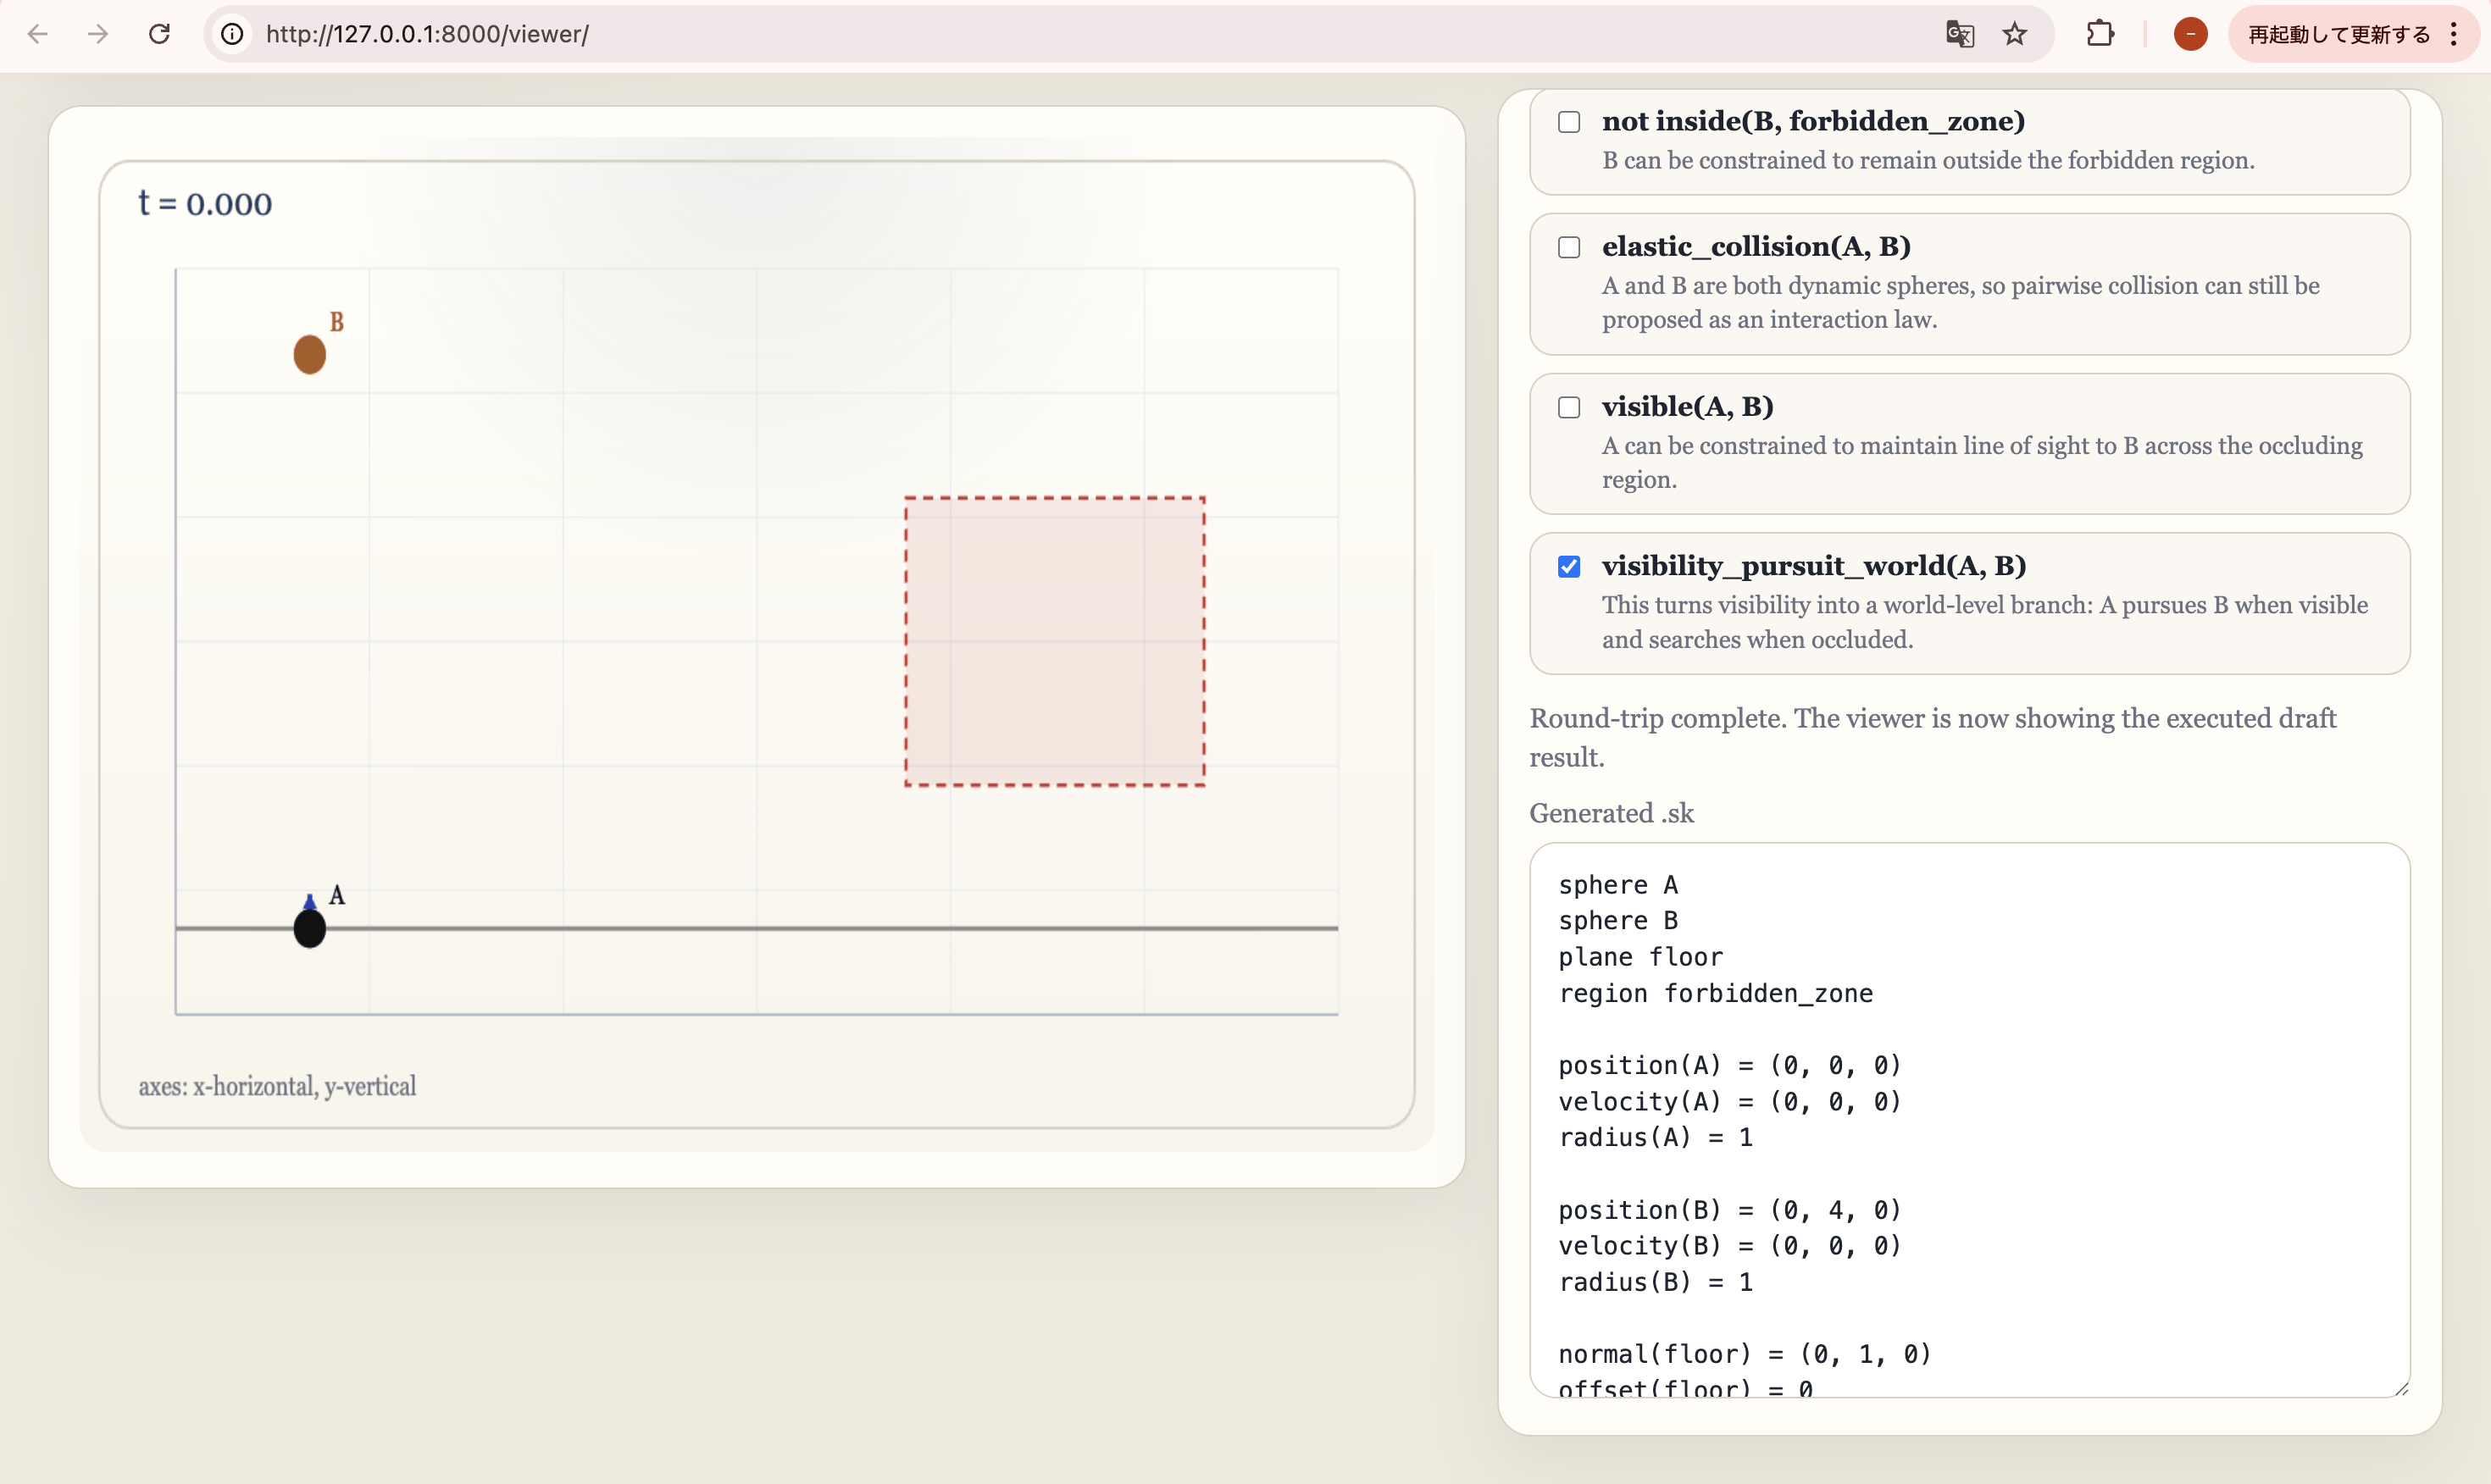
\includegraphics[width=\textwidth]{../figures/viewer-visibility-01-clear-run-paper.png}
  \end{minipage}\hfill
  \begin{minipage}[t]{0.32\textwidth}
    \centering
    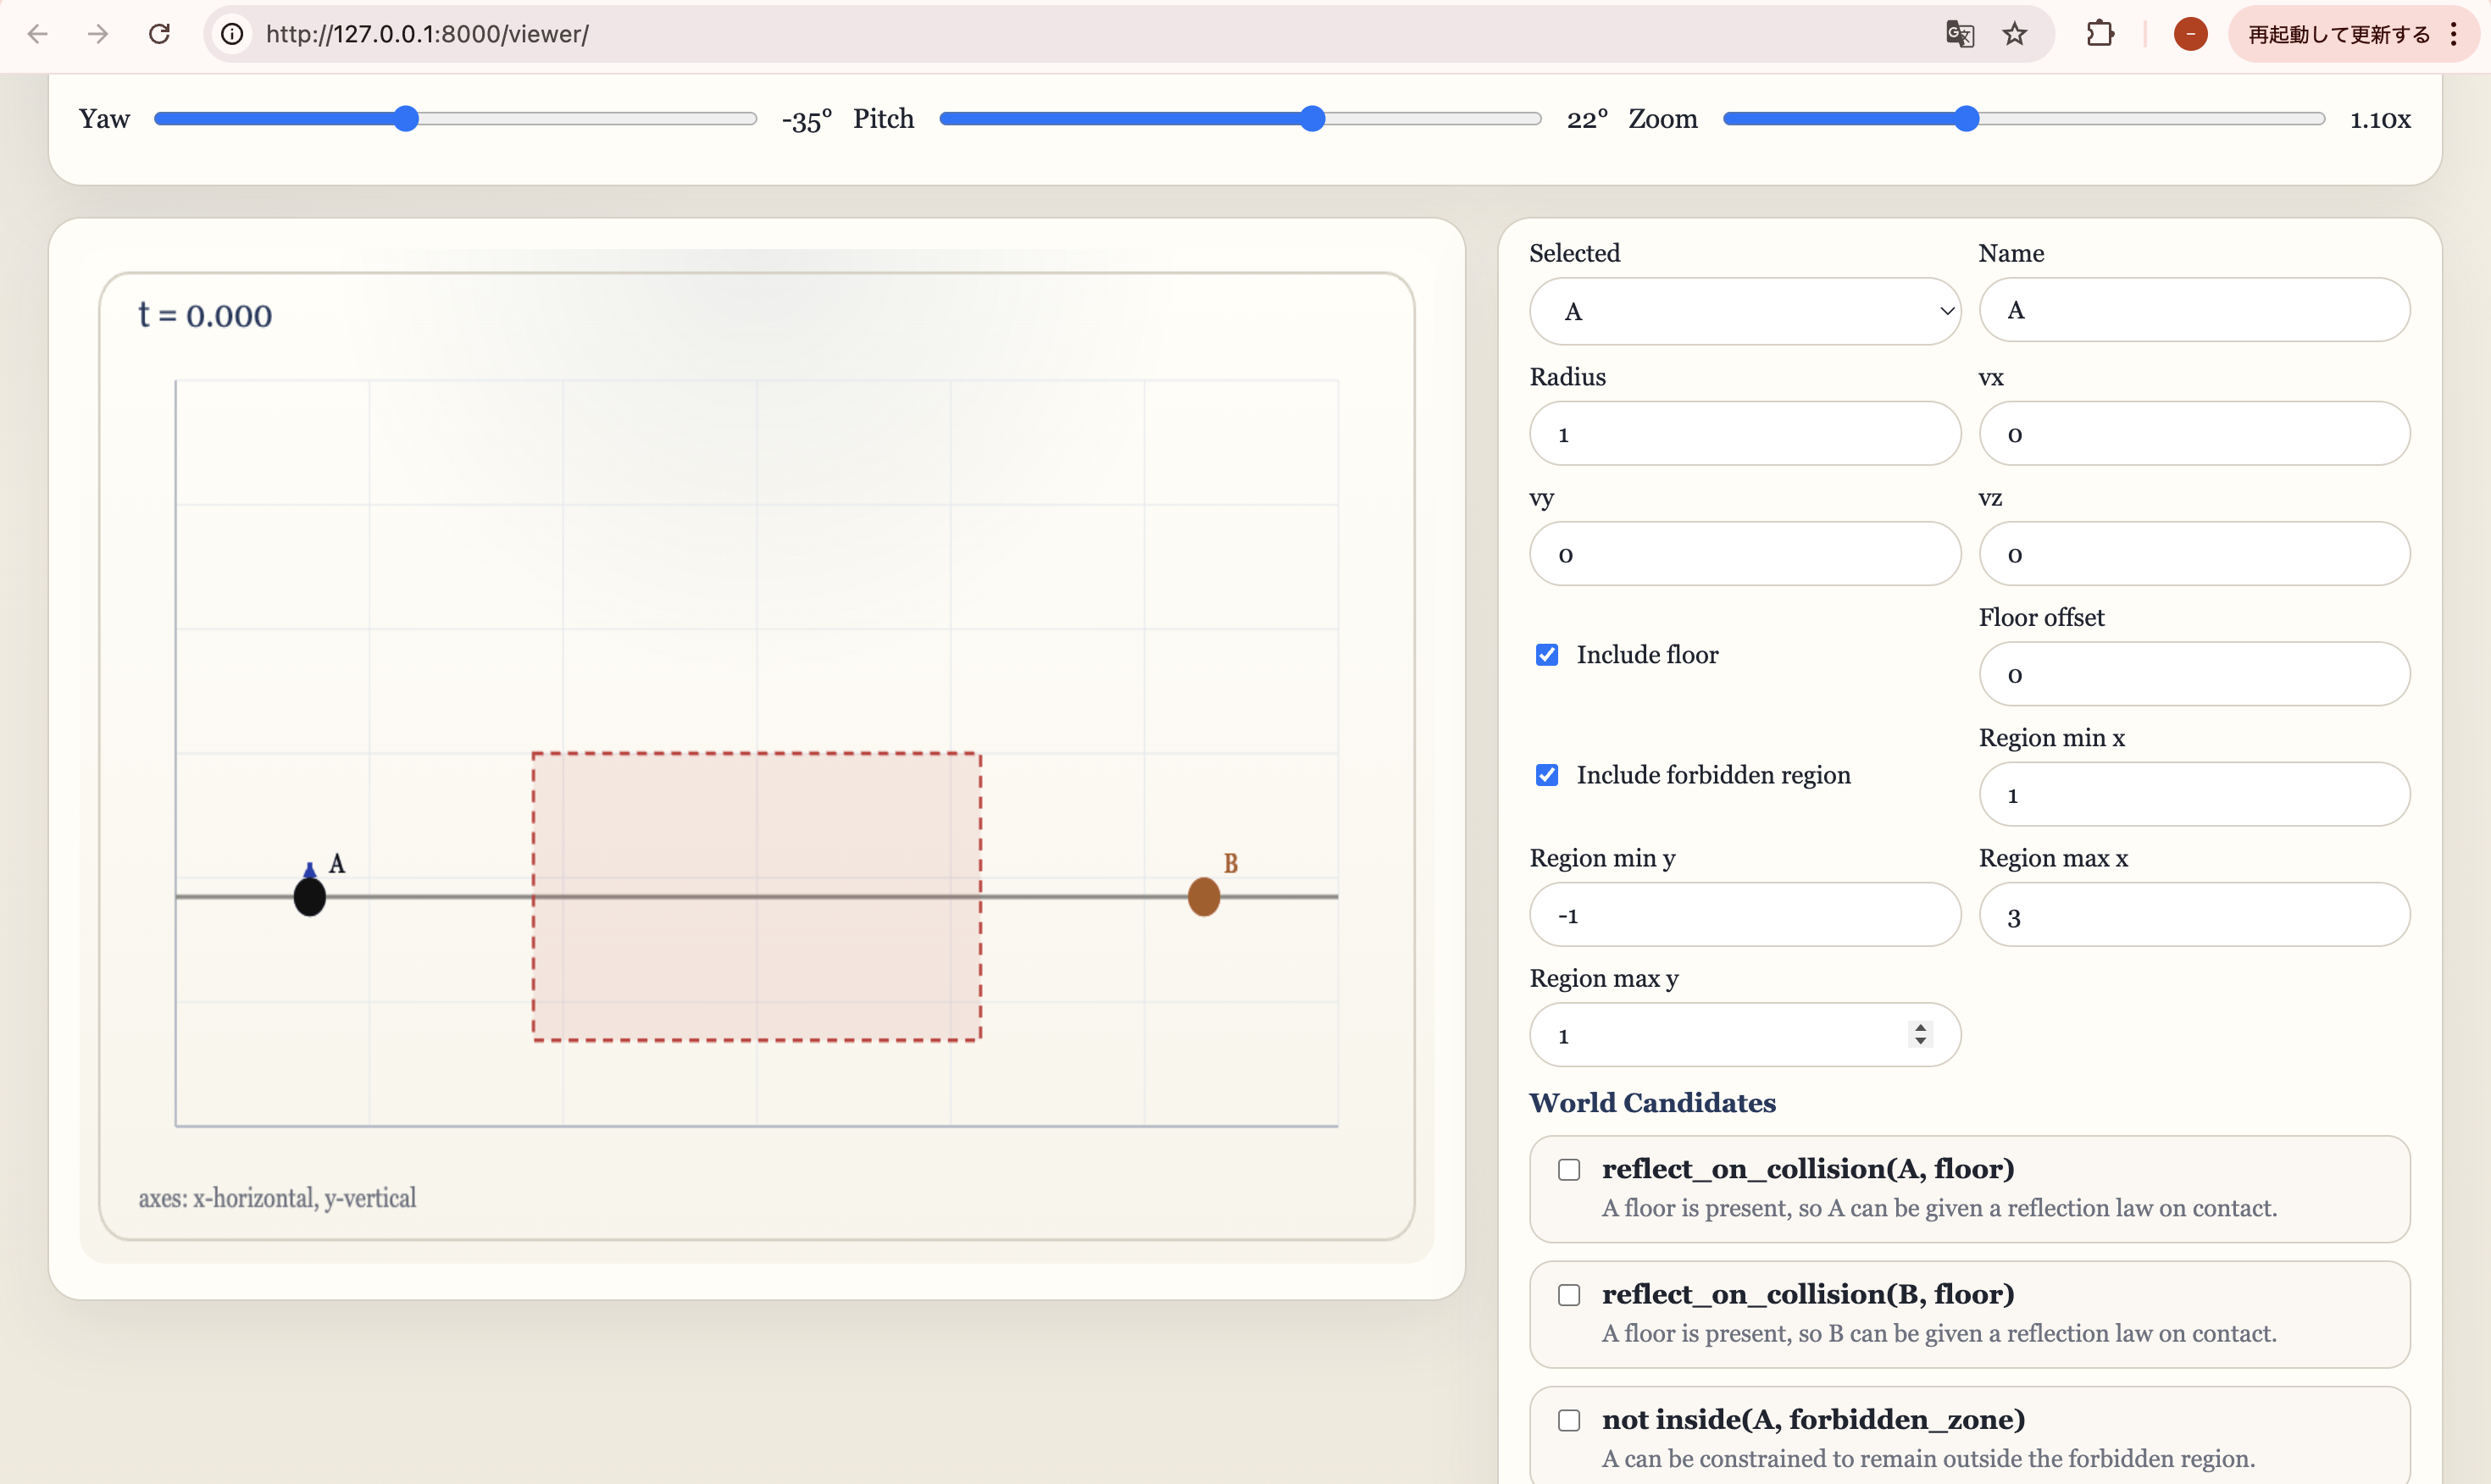
\includegraphics[width=\textwidth]{../figures/viewer-visibility-02-occluded-preset-paper.png}
  \end{minipage}\hfill
  \begin{minipage}[t]{0.32\textwidth}
    \centering
    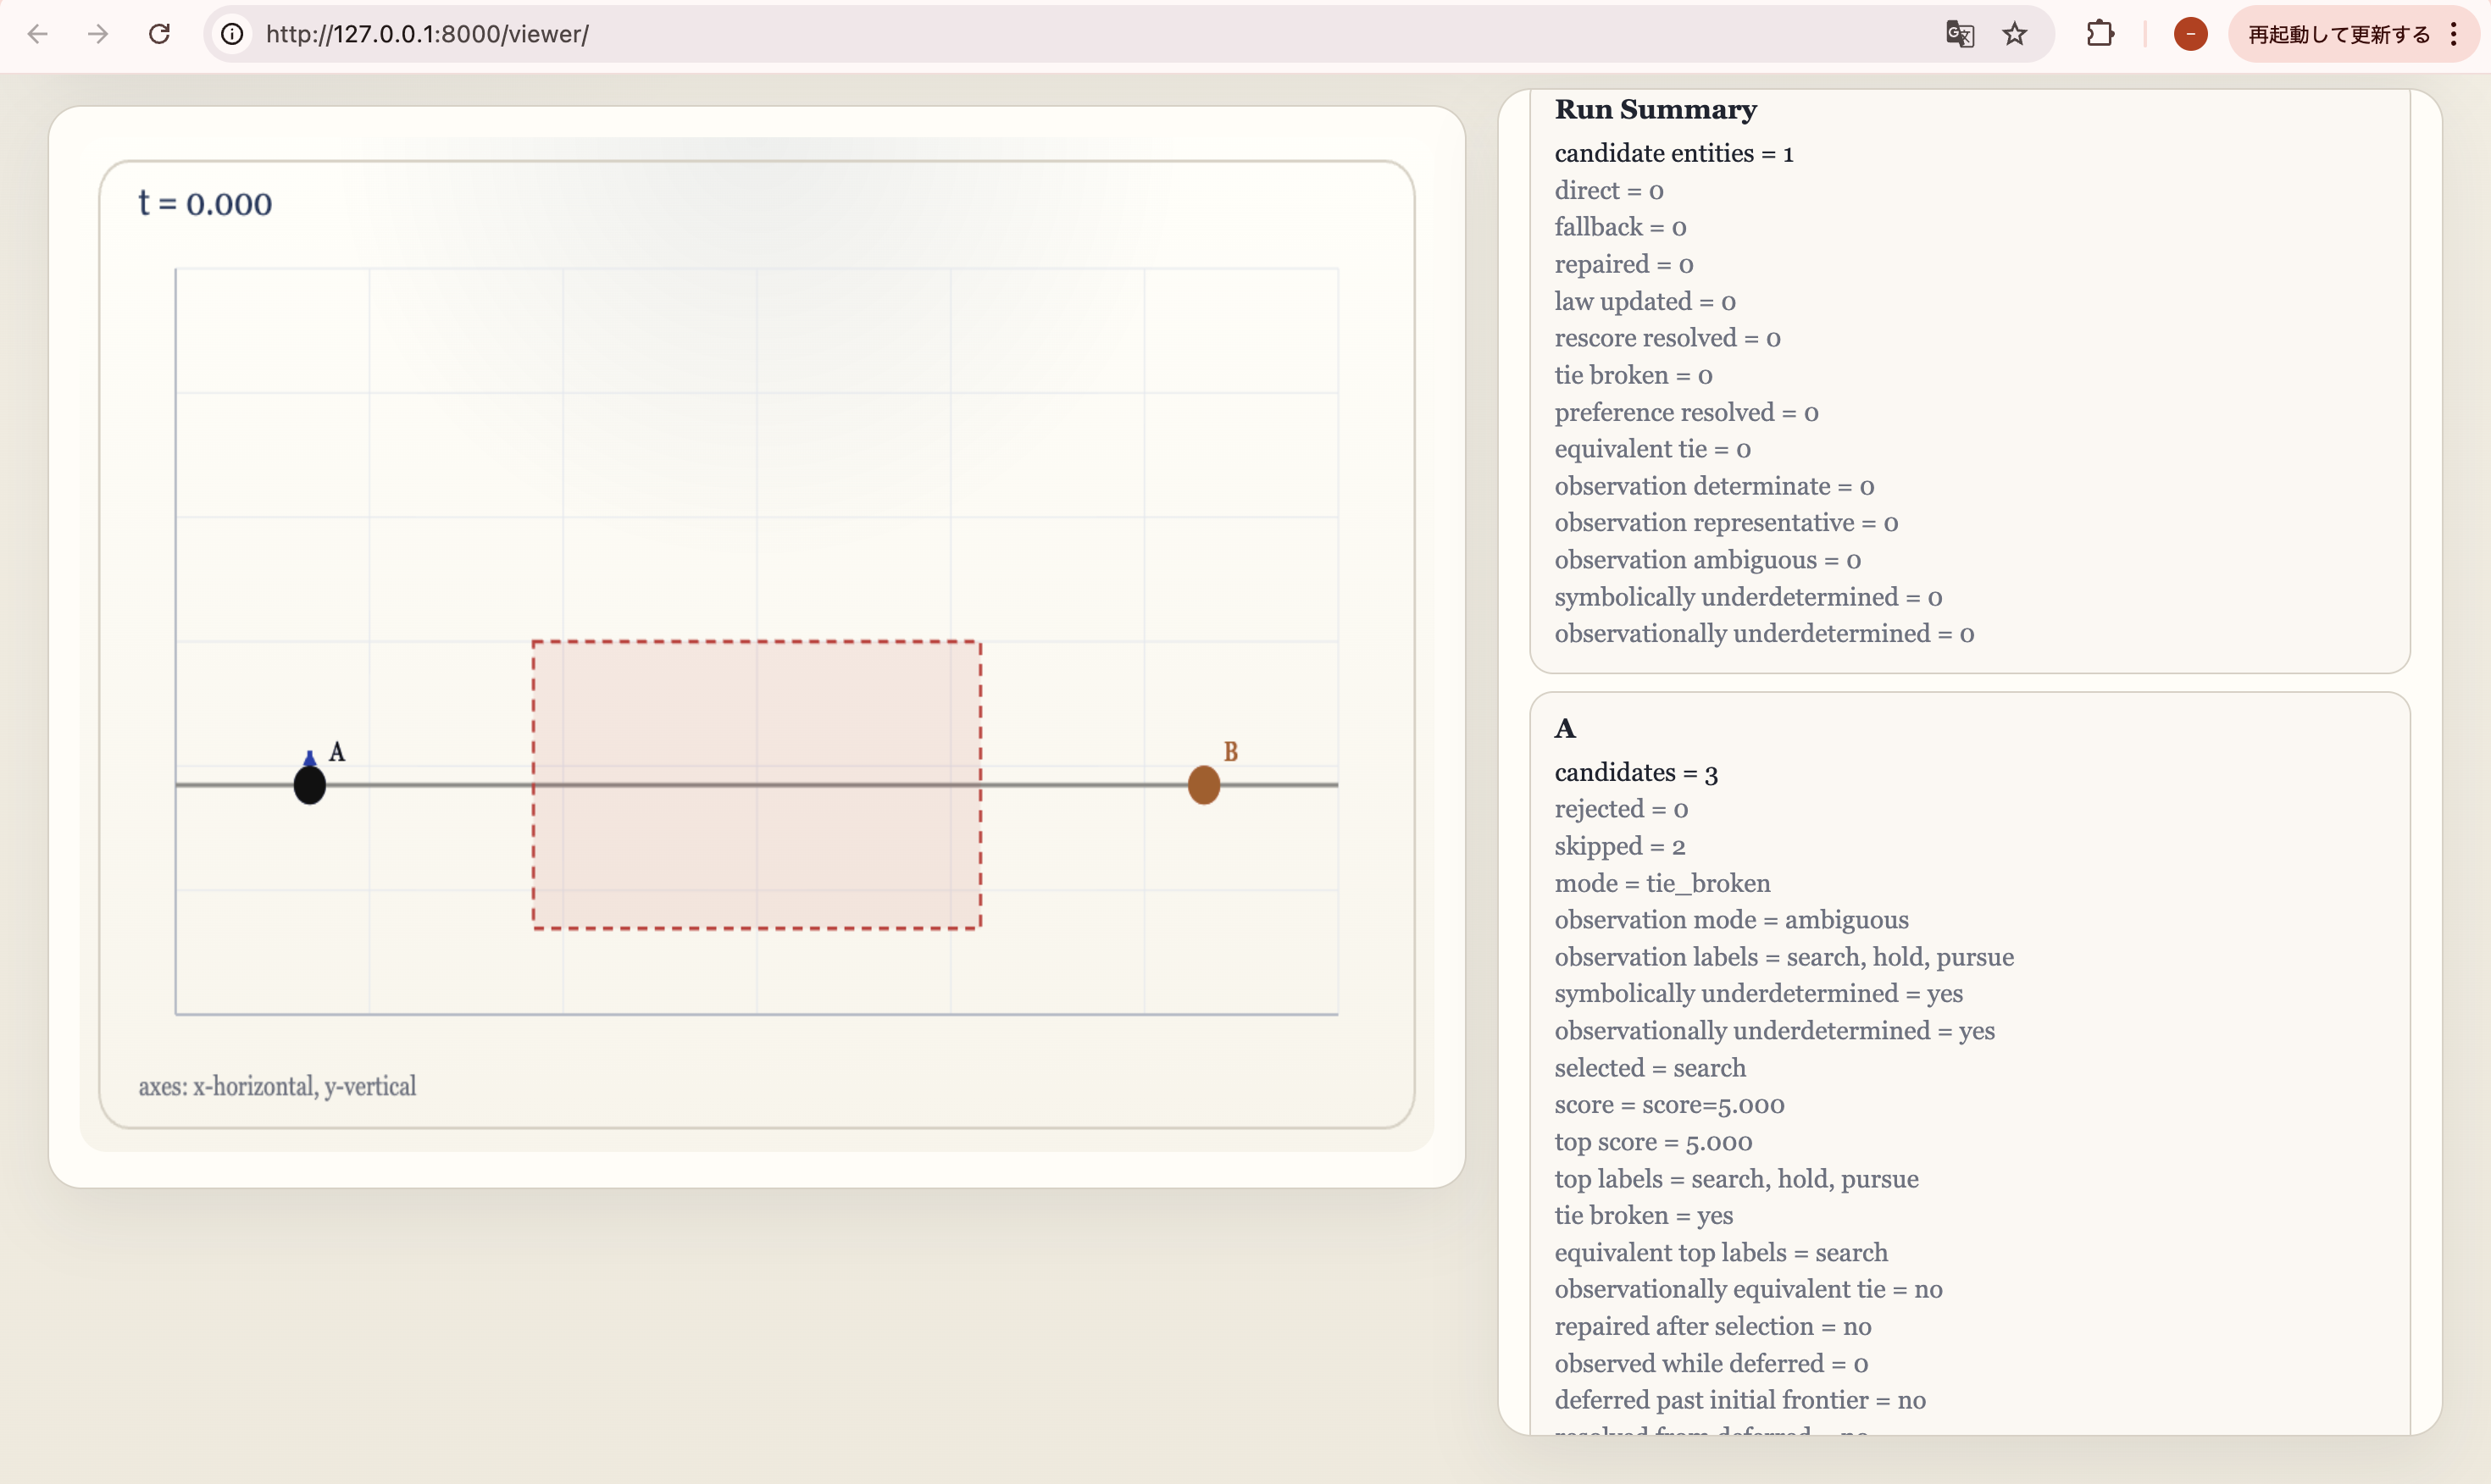
\includegraphics[width=\textwidth]{../figures/viewer-visibility-03-occluded-run-paper.png}
  \end{minipage}
  \caption{Visibility-conditioned world branching in the viewer. Left: a clear-visibility world executes a pursuit-oriented continuation. Center: the draft editor proposes a visibility world with an occluding region. Right: the occluded execution instead selects a search-oriented continuation.}
  \label{fig:visibility-pursuit}
\end{figure*}

\subsection{Early Underdetermined-World Convergence}

The project has also now begun to cross the boundary from fully specified worlds to underdetermined ones.
In a small Phase I extension, a scene can declare multiple candidate velocities for a small finite set of entities together with soft scores, while the existing law layer still acts as a hard admissibility filter.
This produces a useful first convergence model rather than a full search framework.

Two minimal behaviors are already executable.
In the first, the highest-scoring candidate is rejected by a hard law, so the runtime falls back to a lower-scoring admissible candidate.
In the second, the highest-scoring candidate is selected but then repaired by a hard law into an admissible continuation.
The prototype can now also expose top-score ties explicitly, together with the deterministic tie-break that selects one admissible continuation while recording the remaining tied labels as skipped candidates.
It can further distinguish ties whose top-scoring continuations are observationally equivalent, making it explicit when deterministic branch selection chooses a representative continuation rather than an observably different one.
The prototype can now also mix these modes within one world, so one entity may remain deferred while another converges after repair in the same run.
The prototype can also keep a deferred entity unresolved across more than one observed frontier while other entities continue to evolve, and it can later re-converge that entity through a delayed resolution point, a newly active preference, or a later score update.
This convergence work is also starting to connect back to geometry, since a pursuit-like candidate can now be preferred only when another entity remains visible, while an occluded world can prefer a different continuation such as search. That makes line of sight part of world evolution rather than only part of contradiction reporting.
Later law updates can likewise reshape admissibility itself, so a continuation that was previously blocked by a hard law may later become selectable without abandoning the world-oriented formulation.
These re-convergences can also be staggered across multiple entities, so the world-level observation status changes across frontiers instead of collapsing in a single step.
The structured report therefore exposes both the candidate inventory seen before simulation and the candidate resolution performed at the initial frontier, together with run-level convergence analytics covering direct, fallback, repaired, tie-broken, deferred, and observationally equivalent outcomes, as well as whether observation is already determinate, merely representative, or still unresolved in a small executable stand-in for $Obs? = U$.

These additions remain deliberately small, but they matter for the research trajectory.
They show that World-Oriented Programming need not be limited to fully determined evolution.
It can also begin to represent worlds whose next admissible development is chosen through a combination of hard laws and soft preference.

\subsection{What These Results Do and Do Not Show}

The current prototype supports the paper's central conceptual claims.
It shows that declarative world construction can drive execution, that admissibility can be modeled as an explicit world law, that interaction can be localized rather than globally synchronized, and that a first visual-to-execution loop is already implementable.
It also now shows that the same prototype line can be evaluated structurally against compact imperative baselines and extended into a first richer-geometry pillar without abandoning the original world-oriented formulation.

\section{Discussion and Future Work}

The prototype remains intentionally narrow.
Its object vocabulary is small.
Region handling is simplified, simultaneous-event semantics are underspecified, and the visualization pipeline is still far from a mature editor.
The new underdetermined-world slice is likewise intentionally narrow: it currently supports only a small finite set of candidate-bearing entities with one simple scoring model.

These limitations point directly to the next research steps.
One path is implementation-driven: richer geometry, multiple surfaces, bounded plane-built spaces, better simultaneous-event handling, and a stronger diagrammatic interface.
The first geometry slice now underway is a visibility law, where line-of-sight between entities is treated as a world-level condition rather than as ad hoc update logic. The current prototype now also supports multi-occluder visibility, a first corridor-style visibility world, and a first time-varying corridor slice, so line of sight can be shaped by a small declared set of blocking regions and can later change how a deferred world resolves.
The next natural extension is already visible in embryo: multi-target handoff, where geometry steers convergence between several target-specific continuations rather than only between pursuit and search.
The same line of work is now also beginning to show small visibility-driven coordination worlds, where one change in line of sight resolves several deferred entities together.
It is also beginning to show small visibility networks, where the same geometric condition distributes role-specific continuations across several agents.
Those networks are now starting to vary across observation frontiers as well, which suggests a plausible stopping point for this first visibility pillar before moving on to a different geometry family.
That next family is now beginning as a multi-surface slice, where a sphere can evolve between several declared planes under explicit contact laws rather than against a single fixed floor.
It is now also beginning to connect to non-axis-aligned bounded spaces, since a small wedge-shaped admissible volume can already be expressed with two slanted planes and a single \texttt{between\_planes(...)} law.
It is now also beginning to connect bounded spaces to one another, since a small doorway can already be expressed as one wall plane plus one explicit \texttt{through\_gate(...)} law.
It is now also beginning to connect those spaces across time, since one small doorway can already be delayed by an explicit \texttt{through\_gate\_after(...)} law.
It is now also beginning to connect those spaces to branching behavior, since the opening state of that doorway can already be used to prefer \texttt{enter} over \texttt{wait} at a later frontier.
Another path is semantics-driven: extending the current Phase I slice from candidate selection toward a fuller convergence model for underdetermined worlds.
Another path is evaluation-driven: comparisons against imperative baselines, analysis of specification size and clarity, and studies of representational alignment for human users.

Even at its current scale, however, the prototype is already enough to argue that executable world description is not merely a metaphor.
It is becoming a coherent programming model with a runnable core, an emerging semantics, and a first comparative evaluation story.

\bibliographystyle{ACM-Reference-Format}
\bibliography{references}

\end{document}


\end{document}
